\chapter{Overview }\label{Overview}

\section*{A Three-Part Course}

The topics of Calculus II fall into three parts that each have an appropriate place in the story of the calculus sequence.

\begin{itemize}
\item {\bf Part I: Integration.} The first part of the course ties loose ends from Calculus I.  The ending of Calculus I showed that antiderivatives can be used to evaluate integrals via the Fundamental Theorem of Calculus.  However, by the end of Calculus I, only the very simplest antiderivatives can actually be computed.  Part one expands the student's knowledge of {\bf techniques of antidifferentiation}.  These techniques are subsequently put to use computing {\bf length, area, volume, and center of mass}.
\item {\bf Part II: Sequences and Series.} This is the topic that makes up the body of Calculus II.   {\bf Sequences and series} embody the beauty of mathematics; from simple beginnings (a sequence is just a list... a series is just adding up a list of numbers...) it quickly leads to incredible structure, surprises, complexity, and open problems.  {\bf Power series} redefine commonly used transcendental functions (functions that are not computed using algebra, e.g. cosine).  If you've ever wondered {\bf what your calculator does when you press the cosine button}, this is where you find out!  ({\bf Hint:} It does not have a circle of radius one spinning around with a team of elves that measure $x$ coordinates.) %Jenna is still shocked about this....
%with how amazing their fudge cookies are, they're obviously capable of it.  It's just that we're still in contract negotiation regarding wages and benefits.
%Wages right... that explains it. Can't have them overworked at midnight too when students are frantically studying.
% Regarding boldface on the cosine button phrase... basically I want early quick motivation for a student skimming through as to what this stuff is used for.  So that's why I boldfaced the geometric quantities up in part I, and similarly for this in part II.

\item {\bf Part III: Coming Attractions.}  By the end of Calculus II, the student is ready for a \emph{lot} of other classes.  The end of Calculus II thus ends with a sampler platter of topics that show the vast knowledge base built upon the foundation laid in Calculus II.  Here the text takes a bite out of {\bf Differential Equations}, serves some polar and parametric coordinates as a palate cleanser before {\bf Calculus III}, and tastes some {\bf Complex Analysis} to aid in digestion of Differential Equations.  For dessert, it serves a scoop of {\bf Probability} with both discrete and continuous colored sprinkles.
\end{itemize}

\section*{How to Use This Book} This book is meant to facilitate \emph{Active Learning} for students, instructors, and learning assistants.  Active Learning is the process by which the student participates directly in the learning process by reading, writing, and interacting with peers.  This contrasts the traditional model where the student passively listens to lecture while taking notes. This book is designed as a self-guided step-by-step exploration of the concepts.  The text incorporates theory and examples together in order to lead the student to discovering new results while still being able to relate back to familiar topics of mathematics.  Much of this text can be done independently by the student for class preparation.  During class sessions, the instructor and/or learning assistants may find it advantageous to encourage group work while being available to assist students, and work with students on a one-on-one or small group basis.  This is highly desirable as extensive research has shown that active learning improves student success and retention. (For example, see \verb! www.pnas.org/content/111/23/8410! for Scott Freeman's metaanalysis of 225 studies supporting this claim.)
%
\subsubsection*{What is Different about this Book} If you leaf through the text, you'll quickly notice two major structural differences from many traditional calculus books:
%
\begin{enumerate}
\item The exercises are very intermingled with the readings.  Gone is the traditional separation into ``section'' versus ``exercises''.  
\item Whitespace was included for the student to write and work through exercises.  Parts of pages have indeed been intentionally left blank.
\end{enumerate}
%
A consequence of this structure is that the readings and exercise are closely linked.  It is intended for the student to do the readings and exercises concurrently.
\subsubsection*{Ok... Why?}
The goal of this structure is to help the student simulate the process by which a mathematician reads mathematics.   When a mathematician reads a paper or book, he/she always has a pen in hand and is constantly working out little examples alongside and scribbling incomprehensible notes in bad handwriting. 
%
It takes a \emph{long} time and a lot of experience to know how to come up with good questions to ask oneself or to know what examples to work out in order to to help oneself absorb the subject.  Hence, the exercises sprinkled throughout the readings are meant to mimic the margin scribbles or side work a mathematician engages in during the act of reading mathematics.
%
\subsubsection*{The Legend of Coffee}

A potential hazard of this self-guided approach is that while most examples are meant to be simple exercises to help with absorption of the topics, there are some examples that students may find quite difficult.  To prevent students from spinning their wheels in frustration, we have labeled the difficulty of all exercises using coffee cups as follows:

\begin{center}
\tcbox[left=0mm,right=0mm,top=0mm,bottom=0mm,boxsep=0mm,toptitle=0.5mm,bottomtitle=0.5mm,center title,title=Coffee Cup Legend ]
{
	\renewcommand*{\arraystretch}{1.8}%
	\begin{tabular}{l|l|l}
		Symbol & Number of Cups & Description of Difficulty \\ \hline \hline
		
		\Coffeecup & A One-Cup Problem & Easy warm-up suitable for class prep. \\ 
        \Coffeecup \Coffeecup & A Two-Cup Problem & Slightly harder, solid groupwork exercise. \\
        \Coffeecup \Coffeecup \Coffeecup & A Three-Cup Problem & Substantial problem requiring significant effort. \\
        \Coffeecup \Coffeecup \Coffeecup \Coffeecup & A Four-Cup Problem & Difficult problem requiring effort and creativity! \\
	\end{tabular}
}
\end{center}

\newpage

\section*{Glossary of Symbols}

In Precalculus and Calculus I, there is a wide range of how much notation from Set Theory gets used.  To get everyone on the same page, here is a short list of some notation we will use in this text.

\subsection*{Sets and Elements} 

 Often in mathematics, we construct collections of objects called \emph{sets}.  
 \begin{itemize}
 \item  If an object $x$ is in a set $A$, we say $x$ is an \emph{element} of $A$ and write $x\in A $. 
\item If an object $x$ is not in a set $A$, we say $x$ is not an element of $A$ and write $x\not\in A$.
 \end{itemize}
 Any particular object is either an element of a set or it is not.  We do not allow for an object to be partially contained in a set, nor do we allow for an object to appear multiple times in a set.  Often we use curly braces around a comma-separated list to indicate what the elements are.
 \begin{example}{A Prime Example}  Suppose $P$ is the set of all prime numbers.  We write $$P=\lbrace 2,3,5,7,11,13,17,\ldots \rbrace $$ For example, $2\in P$ and $65,537 \in P$, but $4\not\in P$.
 \end{example}

\subsection*{Some Famous Sets of Numbers}
 
 The following are fundamental sets of numbers used in Calculus 2. 
 
 \begin{itemize}
 \item {\bf Natural Numbers:} The set $\mathbb{N}$ of natural numbers is the set of all positive whole numbers, along with zero.  That is, $$\mathbb{N}=\lbrace 0,1,2,3,4,5,\ldots \rbrace $$  Note that in many other sources, zero is not included in the natural numbers. Both are widely used; be aware the choice on this convention will change throughout your mathematical travels!   
 \item {\bf Integers:} The set of integers $\mathbb{Z}$ is the set of all whole numbers, whether they are positive, negative, or zero.  That is, $$\mathbb{Z}=\lbrace \ldots,-4,-3,-2,-1,0,1,2,3,4,\ldots \rbrace $$
 \item {\bf Rational Numbers:} The set of rational numbers $\mathbb{Q}$ is the set of all numbers expressible as a fraction whose numerator and denominator are both integers.
 \item {\bf Real Numbers:} The set of real numbers $\mathbb{R}$ is the set of all numbers expressible as a decimal.
\item {\bf Complex Numbers:} The set $\mathbb{C}$ of complex numbers is the set of all numbers formed as a real number (called the real part) plus a real number times $i$ (called the imaginary part), where $i$ is a symbol such that $i^2=-1$.  
 \end{itemize}
 
\subsection*{Set-Builder Notation}
 The most common notation used to construct sets is \emph{set-builder notation}, in which one specifies a name for the elements being considered and then some property $P(x)$ that is the membership test for an object $x$ to be an element of the set.  Specifically,
$$A=\lbrace x\in B : S(x) \rbrace$$
means that an object $x$ chosen from $B$ is an element of the set $A$ if and only if the claim $S(x)$ is true about $x$.  Sometimes the $``\in B''$ gets dropped if it is clear from context what set the elements are being chosen from.  The set-builder notation above gets read as ``the set of all $x$ in $B$ such that $S(x)$''.  One can think of this as running through all elements of $B$ and throwing away any that do not meet the condition described by $S$.  
 \begin{example}{Interval Notation}  Interval notation can be expressed in set-builder notation as follows:
 
 \begin{itemize}
 \item $(a,b)=\lbrace x\in \mathbb{R}: a<x<b \rbrace$
 \item $[a,b)=\lbrace x\in \mathbb{R}: a\leq x<b \rbrace$
 \item $(a,b]=\lbrace x\in \mathbb{R}: a<x\leq b \rbrace$
 \item $[a,b]=\lbrace x\in \mathbb{R}: a\leq x\leq b \rbrace$
 \end{itemize}
 \end{example}

\begin{example}{Rational, Real, and Complex in Set-Builder Notation }

Set-builder notation is often used to express the sets of rational, real, and complex numbers as follows:
\begin{itemize}
\item $\mathbb{Q}=\left\lbrace \frac{a}{b}: a\in \mathbb{Z}, b\in\mathbb{Z},b\neq 0 \right\rbrace$
\item $\mathbb{R}=\left\lbrace 0.a_0a_1a_2a_3a_4\ldots \times 10^n : n\in \mathbb{N}, a_i\in\lbrace 0,1,2,3,4,5,6,7,8,9\rbrace \textnormal{ where } i \in \mathbb{N} \right\rbrace$  Note this is essentially scientific notation; the concatenation of the $a_i$'s represents the digits in a base-ten decimal expansion. 
\item $\mathbb{C}=\lbrace a+bi: a\in \mathbb{R}, b\in\mathbb{R} \rbrace$

\end{itemize}
\begin{center}
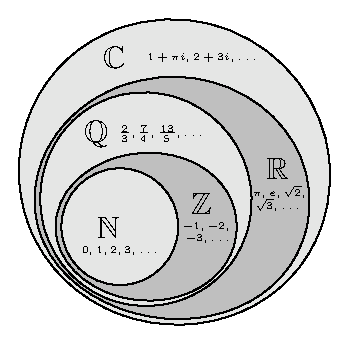
\includegraphics[scale=1]{NumberNotation.eps}
\end{center}
\end{example}